TODO: insert screen-shots

\subsubsection{Basic Interface Structure} % (fold)
\label{ssub:Basic Interface Structure}
The Android user interface is built upon an XML templating engine.
The basic interface is designed via XML templates and later on adapted
and filled with content via Java methods. Every Activity class inherits
from a basic activity class like ``TabActivity'' or ``ListActivity''.
The XML templates define a basic element of the according class also
(``TabHost'', ``ListView'').

% subsubsection Basic Interface Structure (end)

\subsubsection{Main Window} % (fold)
\label{ssub:MainWindow}

The main window is just the skeleton with the tablist, which then
contains the active window itself. The Activities are added
via Intents into the tabbar. An important point, when entering the embedded
Activities into the application's manifest file, is to add the intent filter
\begin{verbatim}
<category android:name="android.intent.category.EMBED"></category>
\end{verbatim}
also. This makes sure, that the Activity respects the boundaries of the
main window when activated.

% subsubsection Main Window (end)

\subsubsection{Dayplan} % (fold)
\label{ssub:Dayplan}
The DayPlan Activity is the basic status interface which shows the current
dayplan in a list. It also contains a context menu for manipulating events
and an application menu to reload events and invoke the optimizer. The
templating for this Activity consists of a template for the ListView and a
separate template for the single rows.

In order create the view, the list of events is fetched from the
ActiveDayPlan. After that a custom ArrayAdapter is used to populate the
single rows of the ListView.
The only slight problem is to get the correct object from the ArrayList,
when tapping a row in the Activity. Fortunately, when the onCreateContextMenu
method is called, it is passed a ContextMenuInfo object as a parameter. This
object contains an id, which is the same as the position in the original
ArrayList from which the view was populated. Therefore it can be used as an
index to identify the correct object in the list. Figure \ref{img:dayplan}
shows an example screen.

\begin{figure}[h!]
    \centering
    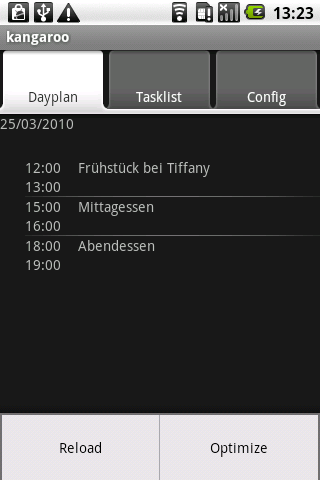
\includegraphics[width=6cm]{pics/gui/main.png}
    \caption{Basic DayPlan with calendar events only}
    \label{img:dayplan}
\end{figure}

% subsubsection Dayplan (end)

\subsubsection{Tasklist} % (fold)
\label{ssub:Tasklist}
The Tasklist Activity displays all the available tasks. It is a two level
list view, which shows the task title in the first level and the task details
on expansion of an entry. It also contains a context menu to manipulate single
tasks and an application menu to add new tasks. The templating for this
Activity is more advanced, as there has to be a template for the ListView
itself, the first level and second level of rows.

The TaskList was slightly more difficult to implement as it is a two-level
ExpandableListView and therefore naturally more complicated. The most important
part is building the entries, as the ListAdapter expects a List of Maps of
Strings to Strings for the first level entries (the task titles) and a List
of List of Maps of Strings to Strings for the second level entries. The
constructor for the adapter (SimpleExpandableListAdapter) then takes these
data structures along with String arrays matching the keys of the passed Maps
and Int arrays containing the IDs of the elements in the respective XML
template for the first or second rows.

\begin{figure}[h!]
    \centering
    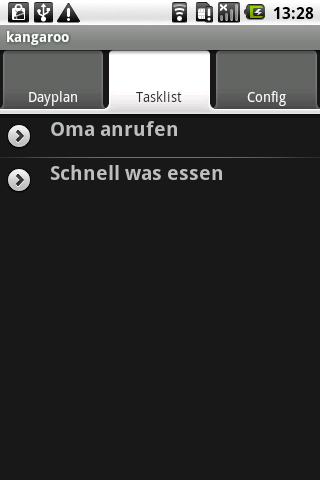
\includegraphics[width=6cm]{pics/gui/task_main.png}
    \caption{}
    \label{}
\end{figure}

% subsubsection Tasklist (end)

\subsubsection{Edit Task} % (fold)
\label{ssub:EditTask}
The EditTask Activity (figure \ref{img:taskedit}) displays information
(title, description, constraints)
of a task object in various edit fields. Here the data can be changed and
is saved on every keystroke. Therefore the data is available when the
Activity is left.

\begin{figure}[h!]
    \centering
    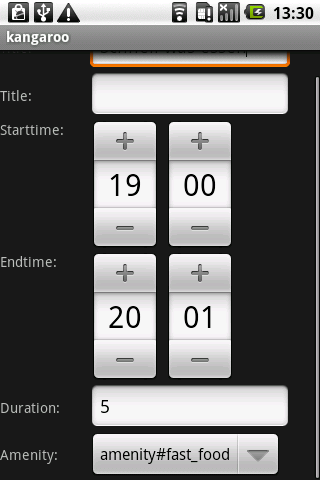
\includegraphics[width=6cm]{pics/gui/task_edit.png}
    \caption{Basic interface for editing tasks}
    \label{img:taskedit}
\end{figure}

% subsubsection Edit Task (end)

\subsubsection{Configuration Editor} % (fold)
\label{ssub:ConfigurationEditor}
The Configuration Activity (figure \ref{img:config}) provides a way to preset several
application
settings, such as calendar name to use and time interval for background
services to do checking. The values are read from and saved to the key-value store
of the kangaroo application. When the application is initially opened, default values
are used.

\begin{figure}[h!]
    \centering
    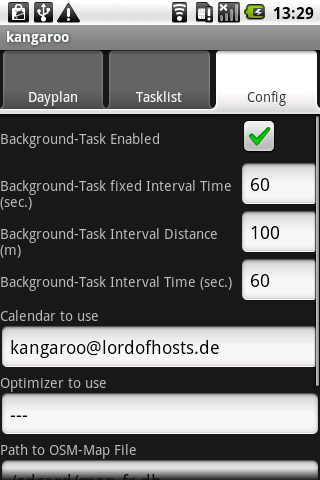
\includegraphics[width=6cm]{pics/gui/config.png}
    \caption{Configuration editor}
    \label{img:config}
\end{figure}

% subsubsection Configuration Editor (end)

\subsubsection{Day Optimizer} % (fold)
\label{ssub:DayOptimizer}
The DayOptimizer Activity (figure \ref{img:dayplanoptimize}) displays a possible
dayplan, optimized via various
characteristics. The user then has the choice whether to accept the new
dayplan, generate a new one or abort. If the dayplan is accepted, it is set
as the current dayplan for the application.

\begin{figure}[h!]
    \centering
    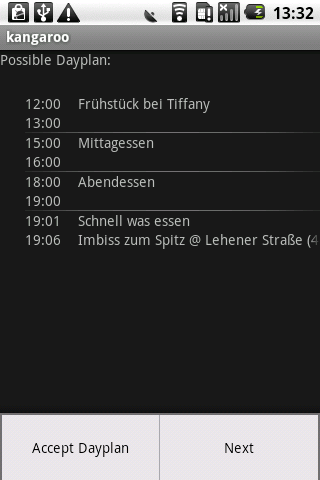
\includegraphics[width=6cm]{pics/gui/optimize_context.png}
    \caption{DayPlan optimizer dialog}
    \label{img:dayplanoptimize}
\end{figure}

% subsubsection Day Optimizer (end)

\subsubsection{Activity Options Menus} % (fold)
\label{ssub:ActivityMenus}
Activity Options Menus are often used to be able to reload an Activity or add
a new element to it. The menu also needs an own XML template, which is
inflated on menu creation. After that, a logic has to be added for every
ID (button) of the menu in the method ``onOptionsItemSelected''.
% subsubsection Activity Menus (end)

\subsubsection{Context Menus} % (fold)
\label{ssub:ContextMenus}
Several context menus are implemented in the various Activities to edit or
delete single objects or provide more information. Context Menus don't have
an XML template for itself, since they are all based on the same layout. Only
the special method ``OnCreateContextMenu'' is needed in the Activity as well
as the registration of the Context Menu via ``registerForContextMenu''.

% subsubsection Context Menus (end)

\subsubsection{Notifications and alerts} % (fold)
The class UserNotification provides an abstraction of the Android user
notifications. The notifications are shown with Kangaroo logo and short message
in the status-bar at the top of the screen (see figure
\ref{img:menubar_notification}). When the user pulls the notification
bar down, a longer text is shown, as shown in figure \ref{img:notifications}.
Upon a click on the text the Kangaroo main GUI is started.
\begin{figure}[h!]
\centering
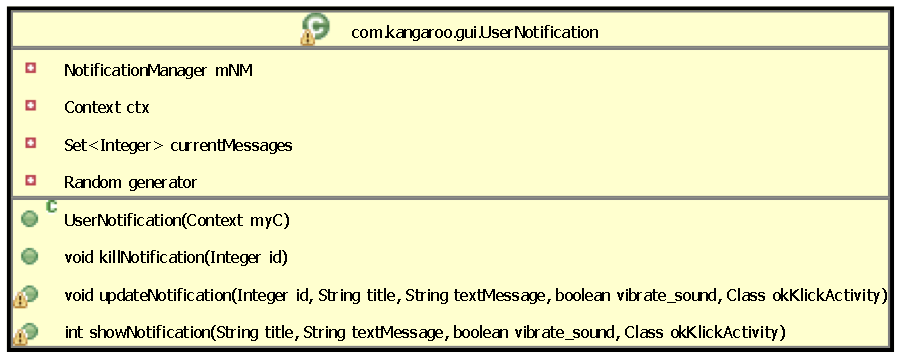
\includegraphics[width=14cm]{pics/notifications.png}
\caption{Class diagram of com.kangaroo.gui.UserNotification}
\label{android_structure}
\end{figure}
The class provides a simple interface. Other parts of the software can initiate
a new notification with the showNotification() method, and are returned an
interger value that represents a unique identifier for this notification. The
caller can decide wether the user should be alerted with a sound and vibrator
alert. With the ID the notification can be deleted or updated with new content.

\begin{figure}[h!]
    \centering
    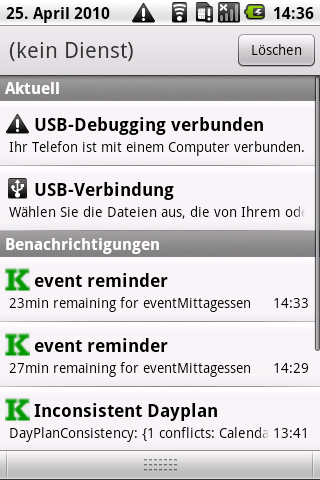
\includegraphics[width=6cm]{pics/gui/notifications_min_late.png}
    \caption{Notifications with longer text}
    \label{img:notifications}
\end{figure}

\begin{figure}[h!]
    \centering
    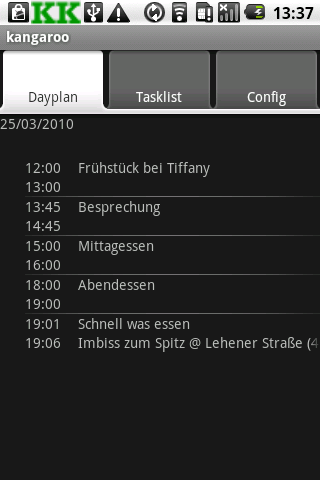
\includegraphics[width=6cm]{pics/gui/menubar_notification.png}
    \caption{Menubar notifications}
    \label{img:menubar_notifications}
\end{figure}
